\pagestyle{plain}
\todo[color=red!40]{Mettre juste la page de références de brainpipe}

% *****************************************************************
%                   BCI MAP
% *****************************************************************
\section{Cartes des Interfaces Cerveau-Machine \citep{graimann_braincomputer_2009}}
\begin{figure}[H]
	\centering
	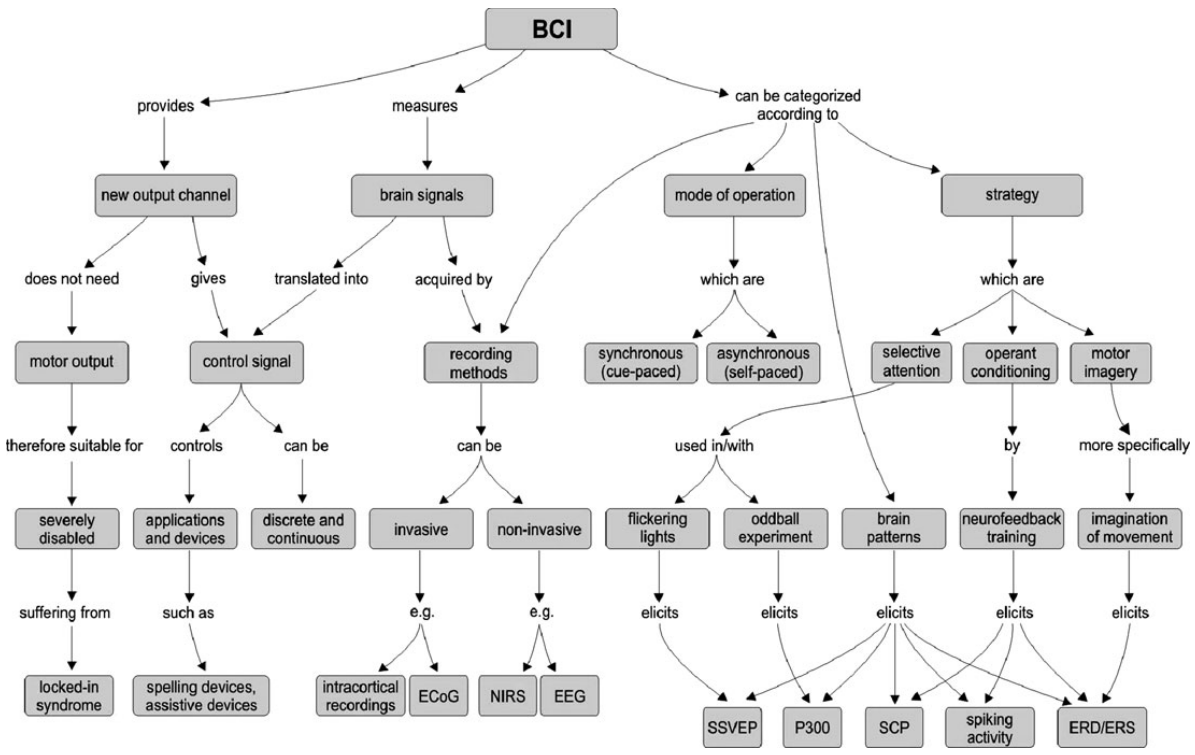
\includegraphics[scale=0.5,angle=-90]{./figures/Grainmann_2002_ICM_map}
	\caption{Cartes des Interfaces Cerveau-Machine \citep{graimann_braincomputer_2009}}
	\label{bci_map}
\end{figure}

% *****************************************************************
%                   BCI COMPETITION
% *****************************************************************
\section{Jeux de donn\'{e}es en libre acc\`{e}s (\textit{BCI competition})}
\begin{figure}[H]
	\begin{tabular}{|c|c|c|p{8cm}|}
		% COMPETITION II
		\hline
		\multicolumn{4}{|c|}{\href{http://www.bbci.de/competition/ii/}{BCI Competition II}} \tabularnewline
		\hline
		Set & N-Classes & Channel & Challenge \tabularnewline
		\hline
		Ia/Ib & 2 & 6-EEG & Decide whether the subject tried to produce cortical negativity or cortical positivity \tabularnewline
		\hline
		IIa & 4 & 64-EEG & Provide the intended target of the feedback test trials  \tabularnewline
		\hline
		IIb & 36 & 64-EEG & Estimate to which letter of a 6-by-6 matrix with successively intensified rows resp. columns the subject was paying attention to  \tabularnewline
		\hline
		III & 2 & 3-EEG & Provide a continuous output that could be used for a BCI- feedback \tabularnewline
		\hline
		IV & 2 & 28-EEG & Predict the laterality of upcoming finger movements (left vs. right hand) 130 ms before keypress \tabularnewline
		\hline

		% COMPETITION III
		\multicolumn{4}{|c|}{\href{http://www.bbci.de/competition/iii/}{BCI Competition III}} \tabularnewline
		\hline
		I & 2 & 64-ECoG & Cued motor imagery (left pinky, tongue) from one subject \tabularnewline
		\hline
		II & 36 & 64-EEG & Estimate to which letter of a 6-by-6 matrix with successively intensified rows resp. columns the subject was paying attention to \tabularnewline
		\hline
		IIIa & 4 & 60-EEG & Cued motor imagery with 4 classes (left hand, right hand, foot, tongue) from 3 subjects. Measure: kappa-coefficient \tabularnewline
		\hline
		IIIb & 2 & 2-EEG & Cued motor imagery with online feedback with 2 classes (left hand, right hand). Measure: mutual information \tabularnewline
		\hline
		IVa/IVb/IVc & 2 & 118-EEG & Cued motor imagery with 2 classes (right hand, foot) from 5 subjects \tabularnewline
		\hline
		V & 3 & 32-EEG & Cued mental imagery with 3 classes (left hand, right hand, word association) from 3 subjects \tabularnewline
		\hline
	
		% COMPETITION IV
		\multicolumn{4}{|c|}{\href{http://www.bbci.de/competition/iv/}{BCI Competition IV}} \tabularnewline
		\hline
		I & 2 & 64-EEG & Motor imagery (2 classes of left hand, right hand, foot) \tabularnewline
		\hline
		IIa & 4 & 22-EEG & Cued motor imagery (left hand, right hand, feet, tongue)   \tabularnewline
		\hline
		IIb & 2 & 3-EEG & Cued motor imagery (left hand, right hand)   \tabularnewline
		\hline
		III & 4 & 10-MEG & Decoding directions of finger/hand/wrist movements \tabularnewline
		\hline
		IV & 5 & 64-ECoG & Discrimination of movements of individual fingers \tabularnewline
		\hline
	\end{tabular}
	\caption{Jeux de donn\'{e}es en libre acc\`{e}s (\textit{BCI competition})}
	\label{annexe_bci_competition}
\end{figure}

% *****************************************************************
%                   COMPARATIF PAC
% *****************************************************************
\section{Comparatif de m\'{e}thodes PAC \citep{tort_measuring_2010}}
\begin{figure}[H]
	\centering
	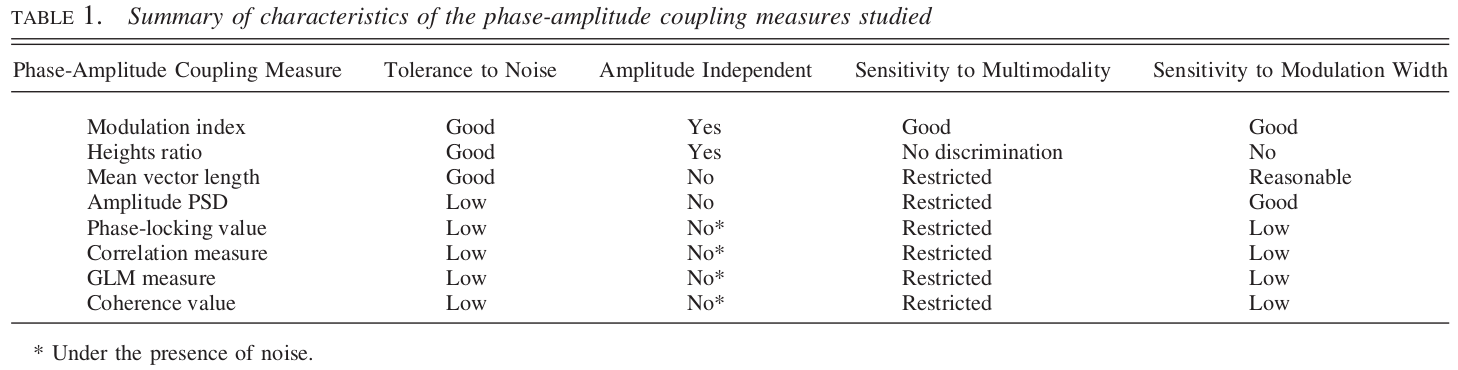
\includegraphics[scale=0.4,angle=-90]{./figures/PAC_methods_comparison}
	\caption{Comparatif de m\'{e}thodes PAC \citep{tort_measuring_2010}}
	\label{comp_pac}
\end{figure}

% *****************************************************************
%                   CLASSIFICATION PIPELINE
% *****************************************************************
\section{Pipeline standard de classification}
\begin{figure}[H]
	\centering
	\makebox[\textwidth][c]{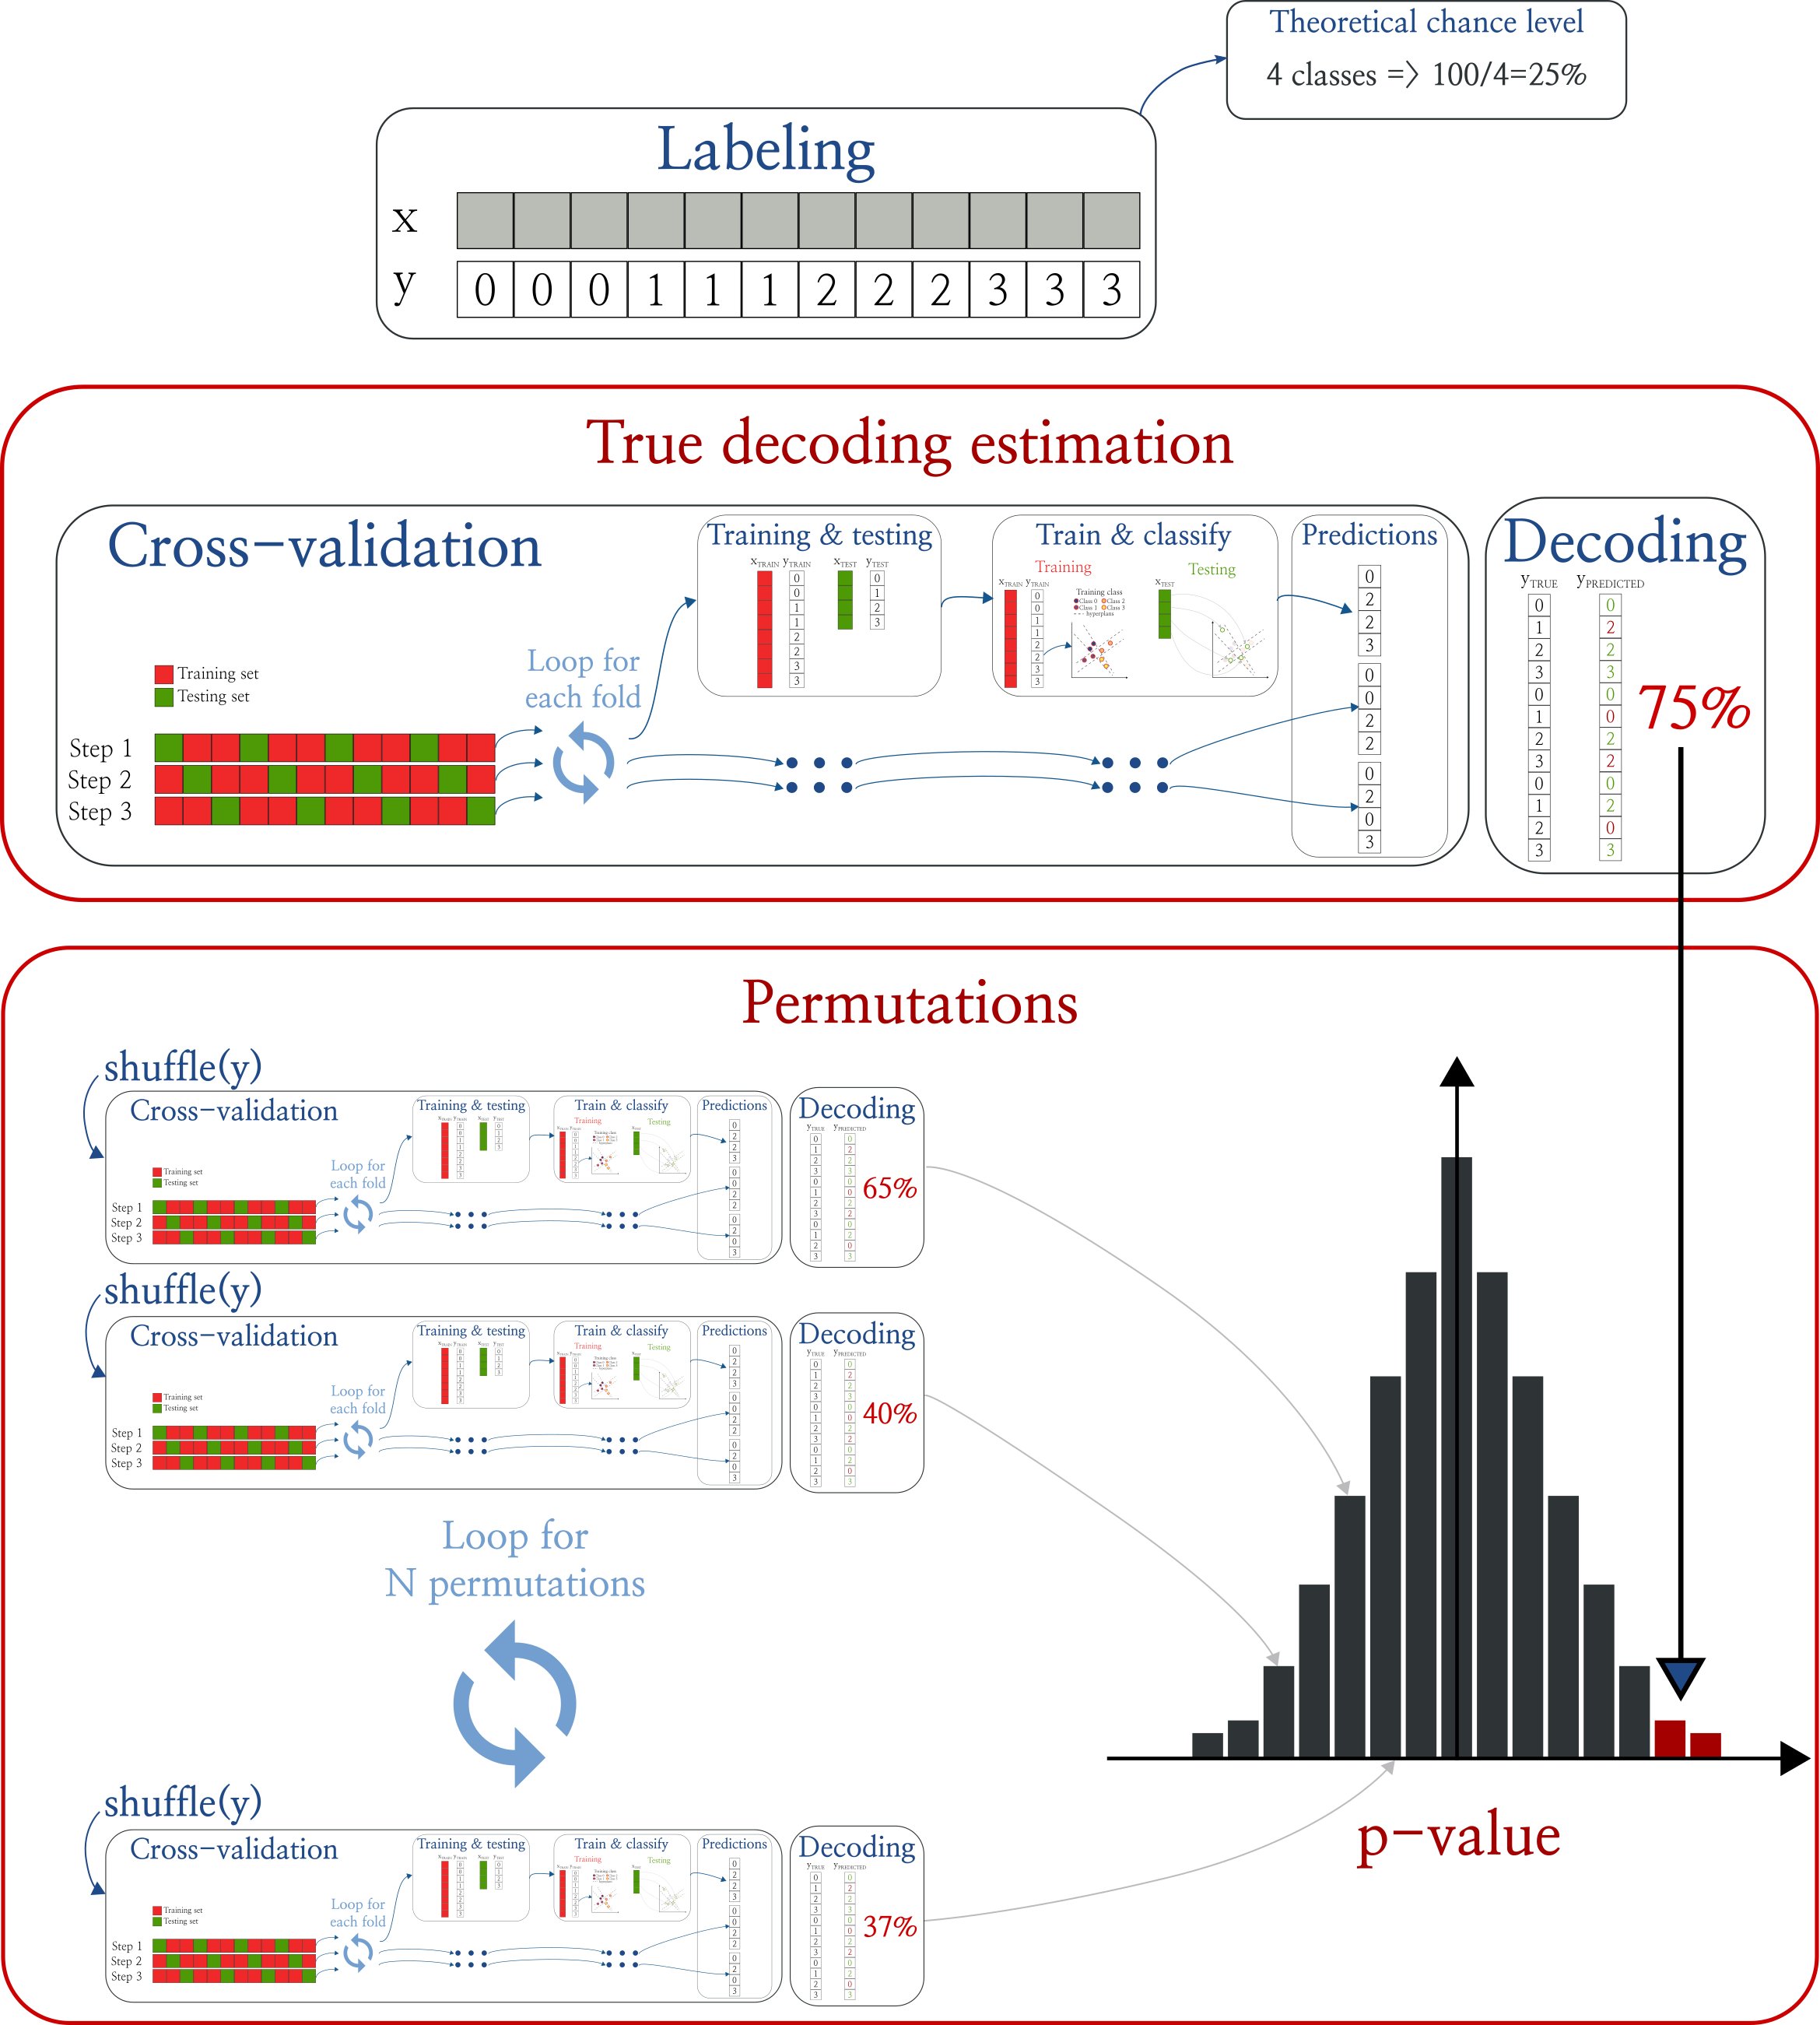
\includegraphics[scale=0.9]{./figures/clf_pipeline}}
	\caption{Pipeline standard de classification}
	\label{clf_pip}
\end{figure}

% *****************************************************************
%                   COMPARATIF CLASSIFIEURS
% *****************************************************************
\section{Comparatif de classifieurs \citep{scikit-learn}}
\begin{figure}[H]
	\centering
	\makebox[\textwidth][c]{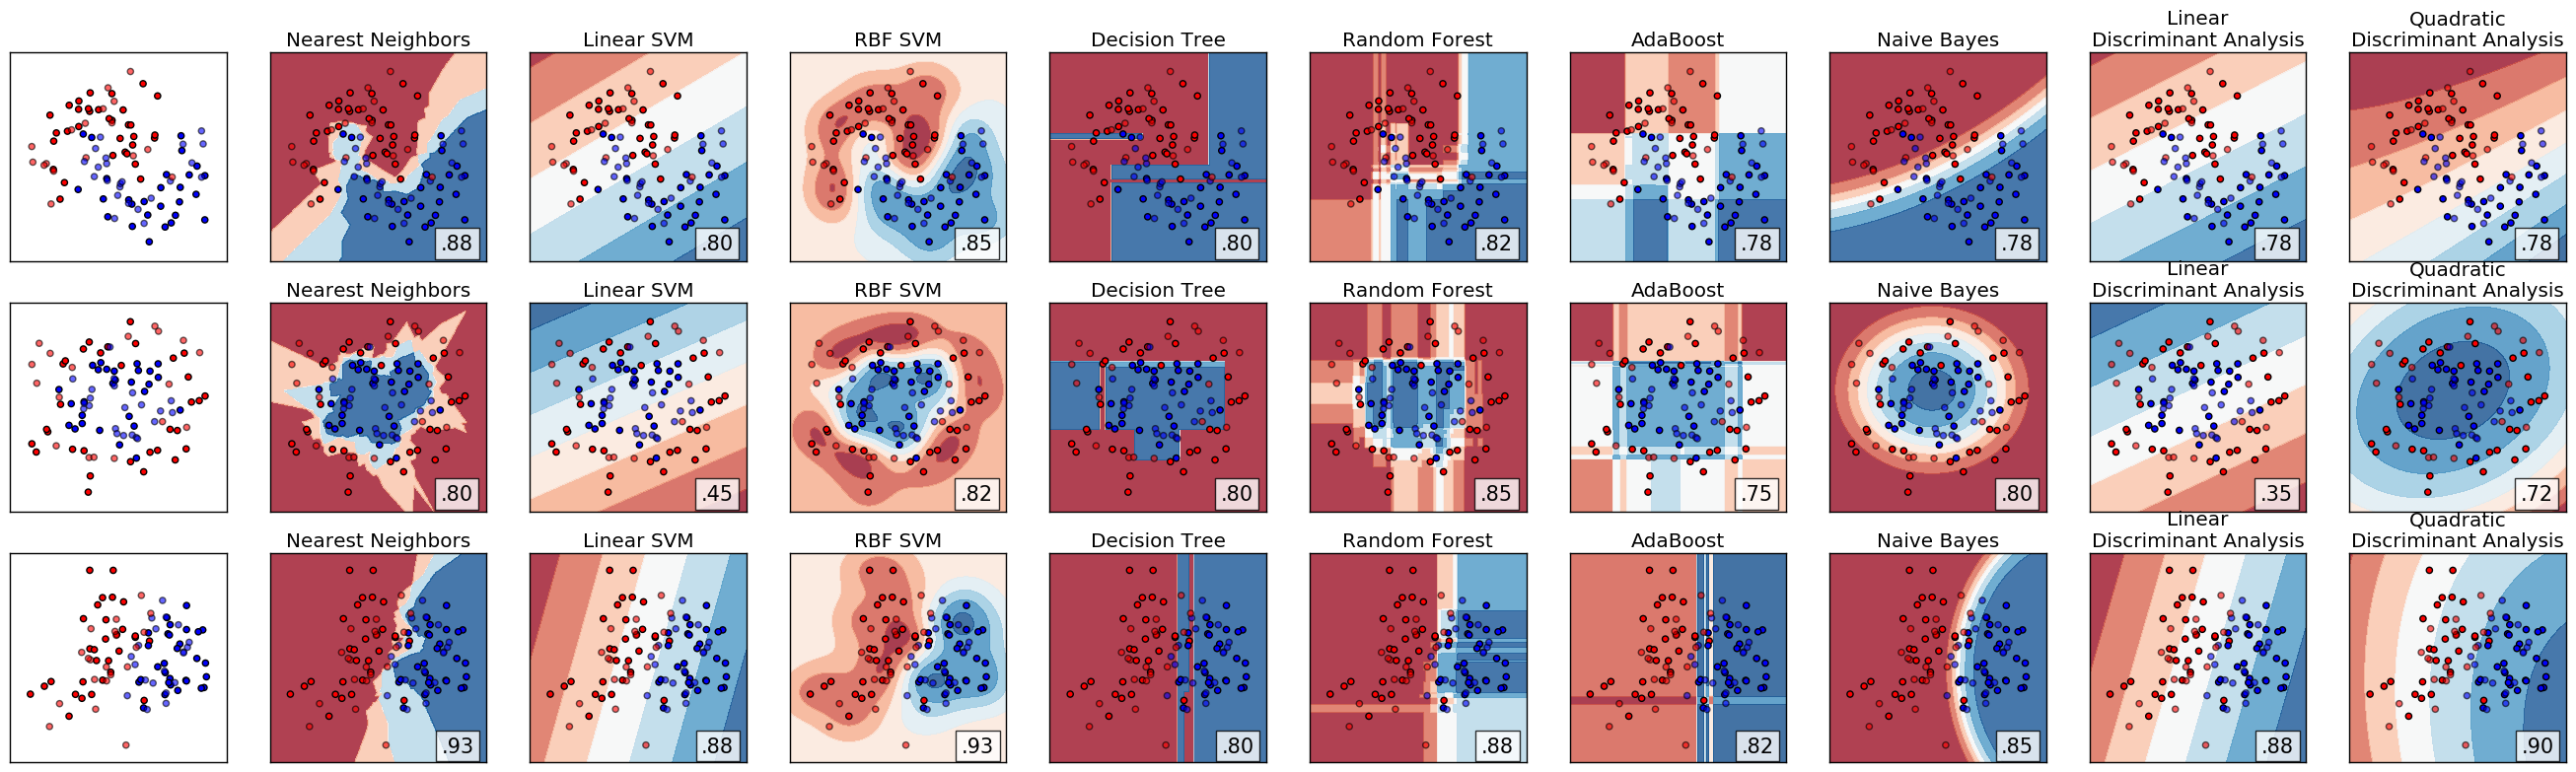
\includegraphics[scale=0.35,angle=-90]{./figures/classifier_comp}}
	\caption{Comparatif de classifieurs \citep{scikit-learn}}
	\label{comp_clf}
\end{figure}


% *****************************************************************
%                   SCHEMA IMPLANTATION
% *****************************************************************
\section{Exemple de sch\'{e}ma d'implantation}
\begin{figure}[H]
	\centering
	\makebox[\textwidth][c]{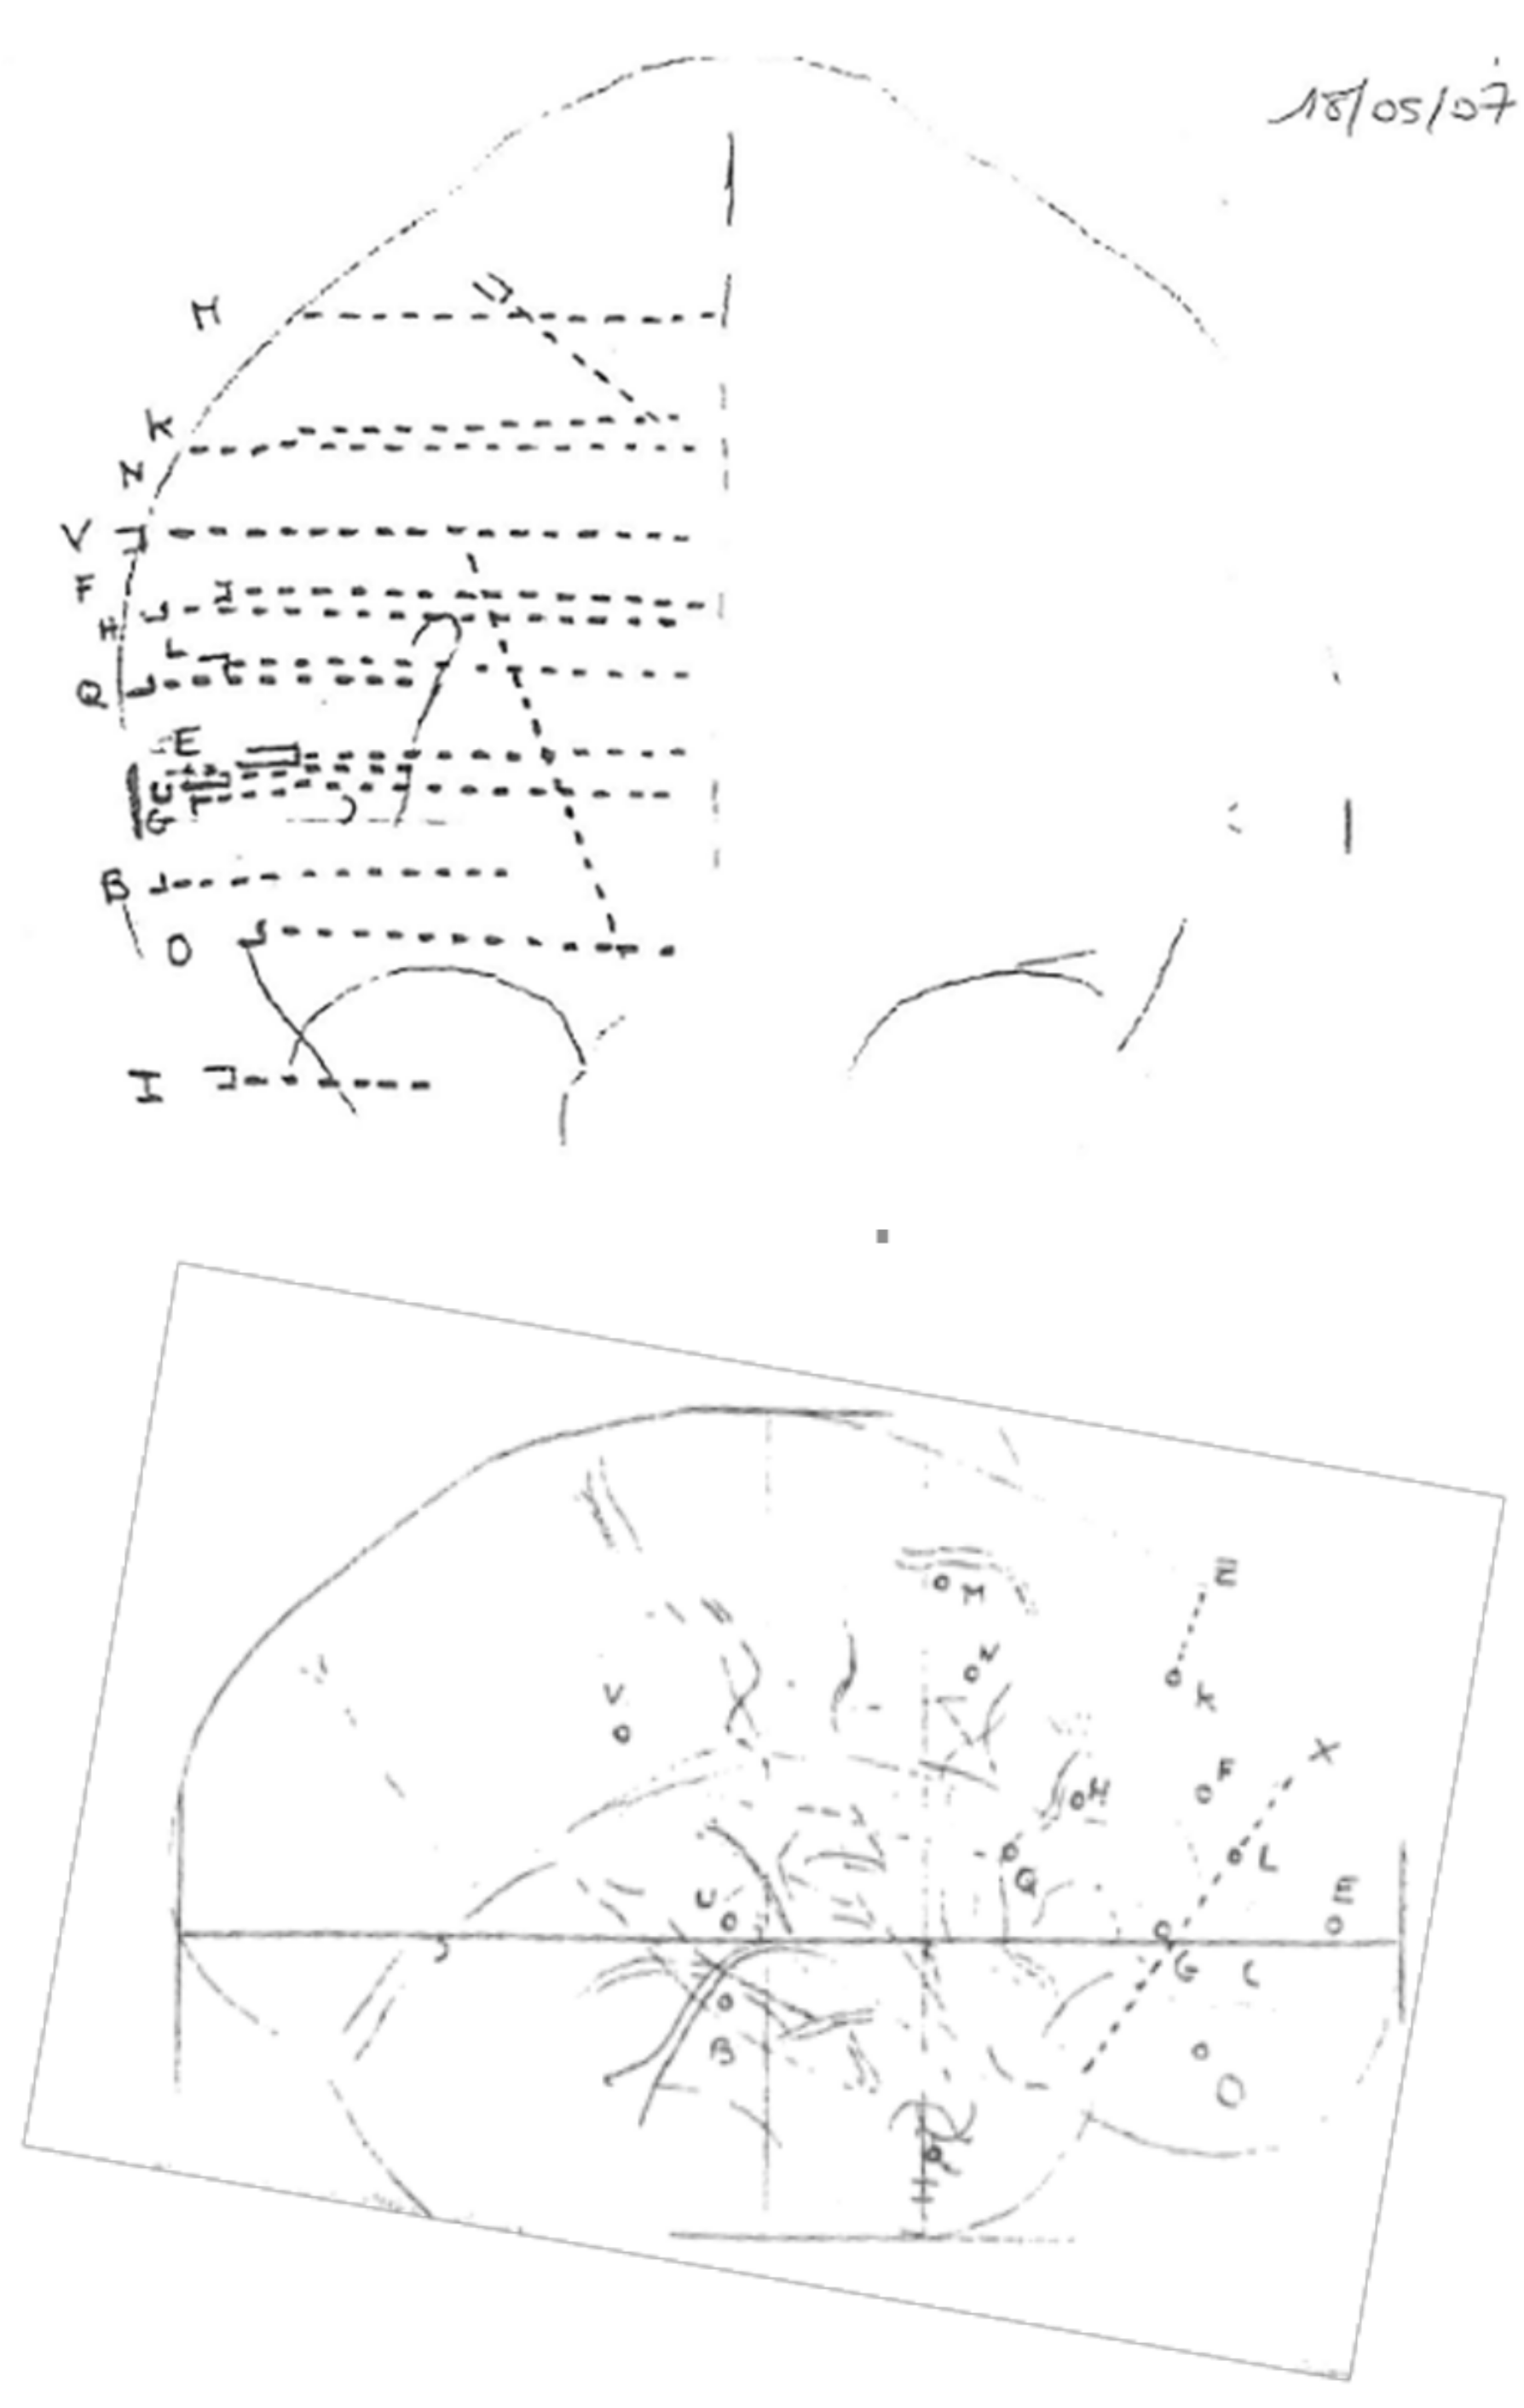
\includegraphics[scale=1]{./figures/schema-implantation_annexe}}
	\caption{Exemple de sch\'{e}ma d'implantation}
	\label{schema_implantation}
\end{figure}
